%%-------------------------------------------------- READ THE COMMENTS CAREFULLY ------------------------------------------%%
%%%%%%%%%%%%%%% Template for generating Report and Presentation according to G.N.D.E.C., Ludhiana's format %%%%%%%%%%%%%%%%%%%%%%%
%% Here myclass is the class name
%% print is used for making a report
%% screen is used for making a presentation
%% If you want the content common in print and screen, then don't specify the content in screen or print environment.
%%----------------------------------------------------------------------------------------------------------------------------
\documentclass[12pt]{myclass}
\usepackage[sectionbreak]{pdfscreen}             %% If you want to produce presesntation then use screen, otherwise use print
%---------------------------------------------------
\usepackage{setspace}
\linespread{1.5}
\usepackage{float}

\renewcommand{\rmdefault}{ptm}				%% font style Times New Roman
\usepackage{titlesec}
\titleformat{\chapter}[display]
    {\normalfont\huge\bfseries}{\chaptertitlename\ \thechapter}{20pt}{\Huge}
\titlespacing*{\chapter}{0pt}{-35pt}{30pt}
%----------------------------------------------------
%%%%%%%%%%%%%%%%%%%% Page Setting %%%%%%%%%%%%%%%%%%%%%%%%%%%

                        %% Here replace your project name
\usepackage[left=2.5cm, right=1.5cm, top=2.5cm, bottom=1.5cm]{geometry}
%\pagestyle{fancy}

%-----------------------------------------%% These commands are used in first page after titlepage
\newcommand{\student}{\vskip 2.5cm}
\newcommand{\supervisor}{\vskip 2cm}
\newcommand{\stamp}{\vskip 2.5cm}                                
%%%%%%%%%%%%%%%%%%%%%%%%%%%%%%%%%%%%%%%%%%%%%%%%%%%%%%%%%%%%%%%%%%%%

%%%%%%%%%%%%%%%%%%%%% Title page %%%%%%%%%%%%%%%%%%%%%%%%%

\uppercase{ \title{e-Notice Application}}
\subtitle{For Android Phones}
\purpose{Synopsis} % or synopsis or Mid term report
\branch{IT} 

\author{Priyanka Kapoor}
\classrollno{106160}
\unirollno{100371180720}

\name{Submitted to which guide} %Prof. Sukhjit Singh Sehra

\branch{Information Technology}     %%INFORMATION TECHNOLOGY


%%----------------------------------------------------------------------%%




%%%%%%%%%%%%%%%%%%%%%%%%%%%%%%%%%%%%%%%%%%%%%%%%%%%%%%%%%%%%%%%%%%%%%%

%%------------------- Body of document----------------------------------%%
\begin{document}


 \maketitle                                 %%% Title page for report


\pagenumbering{Roman}                  %% Pagenumering can be in Roman or arabic

\tableofcontents 
\newpage       %% This command automatically generates Index page
\listoffigures                         %% This command creates a list of figures in the document
\newpage
%\thispagestyle{empty}

\pagenumbering{arabic}                  %% now onwards arabic page numbeing is required
%\cfoot{\thepage}                       %% centered footer (page no.)

%------------------------------------------------------
\section{Introduction}
e-Notice App helps you access online notices on your phone. It is an online notice board maker
where a group of people can easily communicate with each other by sticking virtual notes. These
notes can have text, images or include online videos such as from YouTube.\\
The notice board has always been the place where staff/students gathers to get their latest release
of corporate news. eNotice brings the notice board to a virtual location where staff/students can
not only read notices, but immediately react and respond to them - from their own desks!\\
With this electronic notice and announcement system, email alerts may be sent out notifying
staff that a new notice has been posted, where staff may know if it concerns him directly. In this
way, e-Notice Application also serves as a mailing list for all employees in the directory. This eliminates the
need to keep a separate mailing list which is hard to maintain due to the rapid movement of staff.\\
These are the features that an eNotice App should have:
\begin{itemize}
\item An electronic message board for disseminating information out to staff and students.
\item Notices can be posted, with response obtained instantly.
\item Staff or student can be notified of new postings via email.
\item Notice administrator may push important notices in to selected staff's email.
\item Notice administrator may create any notice category.
\end{itemize}
The interface of this application is straightforward and takes you roughly a minute to get started.
Adding notes to board is easy, just double click on the board and enter the text. Users may also
customize board’s title and background, make board private or public, keep it on “view only”
mode or let everyone post notes.
While registration is not required, users who sign up for an account can keep track of their
boards online. \\
This application can also acts as a market place and lets you advertise, for example, a room to
rent, a car for sale, a job opportunity, a house for sale, an upcoming event, an announcement, a
service, and so on. \\
This application creates interactive notice boards online. You can customize boards with a
custom background, title and background images. It allows users to add sticky notes with text,
images and videos. You can set preferences on who can edit and view the board. Facility of drag
and drop notes anywhere on the board is available. Users can sign using their Google accounts /
Facebook Account and can share boards with others.

%-----------------------------------------------------------
\section{Objective}
The proposed system's objectives are to overcome all the limitations and drawbacks of the
existing system. The online 'e-Notice' application is user-friendly android application. The main
objective of the application is its simplicity of design and ease of implementation that shows and
helps to collect most of the information about events going on in college premises. The interface
will be very user-friendly. \\
The main objectives of the proposed system can be enumerated as follows:
\begin{itemize}
\item Faster dissemination of notices regarding education, technical events, cultural events or
\item Any lost/ found going out in college.
\item Easy way to broadcast your message.
\item Helps you to be updated with whats going on in College.
\item Good way to advertise about Tuitions/ Coaching and Courses.
\item User can also follow a group notice board.
\end{itemize}

%-------------------------------------------------
\section{Technical Details}
\textbf{Languages used:}

\begin{itemize}
\item \textbf{\emph{XML:}} It is used for Designing purpose.
\item \textbf{\emph{Core Java:}} It is used for Logic building.
\end{itemize}
\textbf{Operating Systems:}
\begin{itemize}
\item Android
\item Ubuntu
\end{itemize}
\textbf{Database:}
\begin{itemize}
\item SQLite
\item MySQL
\end{itemize}
\textbf{IDE (Integrated Development Environment):}
\begin{itemize}
\item Eclipse
\item gEdit
\end{itemize}
\textbf{Web Service:}\\
Web Services supports communication between two electronic devices over World Wide Web.


\section{Innovation and Usefulness}
The innovative idea behind this project is to make a physical notice board virtual, that can be
viewed anytime and anywhere immediately at the time when it is posted. This application also
helps to maintain the record of previous notices. You can make various groups like College
Notices, Event Notices of Societies, Library Notices, Placement Regarding Notices and many
other. The user subscribed to any group will get notify when any new notice is posted on it. User
can also respond to the notice if require.\\ 
This application has many uses. It cannot be used in college only but can also be used in Office
Places. It can also act as a market place by advertising about the various products and
technologies.

\begin{figure}[H]
\centering 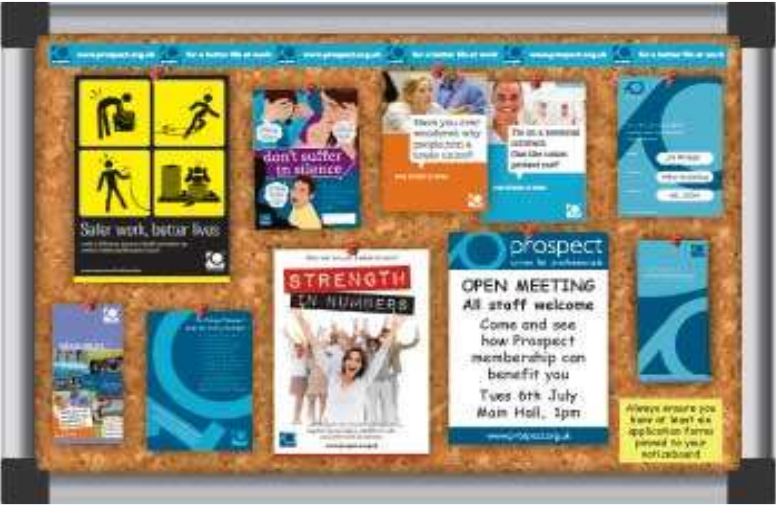
\includegraphics[scale=0.5]{image/notice.png}
\caption{DashBoard of Notices}
\end{figure}
\subsection{Features of Application}
\begin{enumerate}
\item \textbf{\emph{Sign In Using Google or Facebook Accounts:}}\\
 There is no need of registering for this
application. User can use his or her Google or Facebook account to login into this application. So
it relaxes you from learning new id and password.
\item \textbf{\emph{Sticky Notes:}}\\
User also have sticky notes facility through which a user can make a note of any
useful notice while reading the noticeboard. It will help him/her in remembering any of the
useful information regarding events going on in the college.
\item \textbf{\emph{Drag and Drop Notes:}}\\
It also allows you to drag and drop any PDF file, image or a video to
a vitual board that can be viewed by all. It helps and save you from writing lengthy notices again
and again.
\item \textbf{\emph{Customized Boards:}}\\
In this application, user can change the color of notice board or can
apply a decent background of his/her own choice.
User Preferences: User can also set who all can view the notice and who all can edit or post
the notices. The entire work will be under the control of admins of various groups and
departments.
\end{enumerate}


\section{Current Status Of Project}

This section describes the project as per the various stages of the Software Development life
cycle. The model of software development life cycle used in this project is the waterfall method.
The Waterfall Method is comprised of a series of very definite phases, each one run intended to
be started sequentially only after the last has been completed, with one or more tangible
deliverables produced at the end of each phase of the waterfall method of SDLC. Essentially, it
starts with a heavy, documented, requirements-planning phase that outlines all the requirements
for the project, followed by sequential phases of design, coding, test-casing, optional
documentation, verification (alpha-testing), validation (beta-testing), and finally
deployment/release.\\
\begin{figure}[H]
\centering 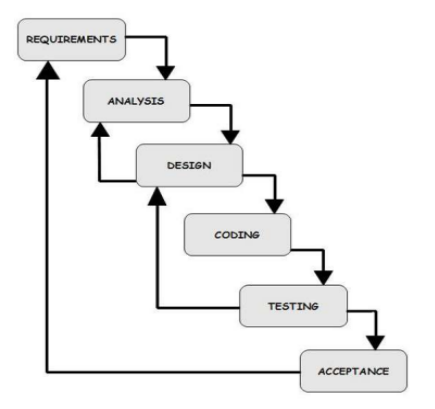
\includegraphics[scale=0.5]{image/sdlc.png}
\caption{Modified Waterfall Model}
\end{figure}

As shown in the Figure, the Waterfall model contains the following stages of software
development:
\begin{enumerate}
\item Requirement Analysis
\item Design
\item Implementation
\item Testing
\item Maintenance
\end{enumerate}
\begin{enumerate}
\item \textbf{\emph{Requirement Analysis:}}\\
Existing system is time consuming and it makes difficult to convey huge amount of users about
any event, class or seminar almost instantly. Also there is always a big crowd in front of
noticeboard. So it was hectic to read any useful instruction and information. Thus all the
problems of the existing system are summarized and proposing a new system that works as an
online application. It is a value added solution to the problem. It resolves all the problems stated
above. It will provide simple interface to the user to operate on and convey the intended users
about events almost instantly, anytime and anywhere.\\
Rests of the above stages of SDLC are under process.
\end{enumerate}


\end{document}
%%------------------------End document-------------------------%%
